\documentclass[9pt,twocolumn,twoside,lineno]{pnas-new}

%% Some pieces required from the pandoc template
\providecommand{\tightlist}{%
  \setlength{\itemsep}{0pt}\setlength{\parskip}{0pt}}

% Use the lineno option to display guide line numbers if required.
% Note that the use of elements such as single-column equations
% may affect the guide line number alignment.

\usepackage[T1]{fontenc}
\usepackage[utf8]{inputenc}

% load packages
\usepackage{float}
\usepackage{listings}
\lstset{numbers=left}

% define struts for tables
\newcommand\T{\rule{0pt}{2.6ex}} %top strut
\newcommand\B{\rule[-1.2ex]{0pt}{0pt}} % bottom strut

\templatetype{pnasresearcharticle}  % Choose template

\title{Environmental and geographic variables are effective surrogates for
genetic variation in conservation planning}

\author[a,1]{Jeffrey O. Hanson}
\author[b]{Jonathan R. Rhodes}
\author[a]{Cynthia Riginos}
\author[a]{Richard A. Fuller}

  \affil[a]{School of Biological Sciences, The University of Queensland, Brisbane,
QLD, Australia}
  \affil[b]{School of Earth and Environmental Sciences, The University of
Queensland, Brisbane, QLD, Australia}


% Please give the surname of the lead author for the running footer
\leadauthor{Hanson}

% Please add here a significance statement to explain the relevance of your work
\significancestatement{To protect biodiversity for the long term, nature reserves and other
protected areas need to represent a broad range of different genetic
types. However, genetic data are expensive and time consuming to obtain.
Here we show that freely available environmental and geographic
variables can be used as effective surrogates for genetic data in
conservation planning. This means that conservation planners can, with
some confidence, design protected area systems to represent
intra-specific genetic diversity without investing in expensive
programmes to obtain and analyze genetic data.}


\authorcontributions{JOH performed the analyses. All authors developed the study and drafted
the manuscript.}

\authordeclaration{The authors declare no conflict of interest.}


\correspondingauthor{\textsuperscript{1} To whom correspondence should be addressed: E-mail: jeffrey.hanson@uqconnect.edu.au.}

% Keywords are not mandatory, but authors are strongly encouraged to provide them. If provided, please include two to five keywords, separated by the pipe symbol, e.g:
 \keywords{  conservation |  biodiversity |  AFLP |  genetic diversity   }

\begin{abstract}
Protected areas buffer species from anthropogenic threats and provide
places for the processes that generate and maintain biodiversity to
continue. However, genetic variation, the raw material for evolution, is
difficult to capture in conservation planning, not least because genetic
data require considerable resources to obtain and analyze. Here we show
that freely available environmental and geographic distance variables
are highly effective surrogates in conservation planning for
representing adaptive and neutral intra-specific genetic variation. We
obtained occurrence and genetic data from the IntraBioDiv project for 27
alpine plant species collected over the European Alps using a gridded
sampling scheme. For each species, we identified loci that were
potentially under selection using outlier loci methods, and mapped their
main gradients of adaptive and neutral genetic variation across the grid
cells. We then used the cells as planning units to prioritize protected
area acquisitions. First, we verified that the spatial patterns of
environmental and geographic variation were correlated, respectively,
with adaptive and neutral genetic variation. Second, we showed that
these surrogates can predict the proportion of genetic variation secured
in randomly generated solutions. Finally, we discovered that solutions
based only on surrogate information secured substantial amounts of
adaptive and neutral genetic variation. Our work paves the way for
widespread integration of surrogates for genetic variation into
conservation planning.
\end{abstract}

\dates{This manuscript was compiled on \today}
\doi{\url{www.pnas.org/cgi/doi/10.1073/pnas.XXXXXXXXXX}}

\begin{document}

% Optional adjustment to line up main text (after abstract) of first page with line numbers, when using both lineno and twocolumn options.
% You should only change this length when you've finalised the article contents.
\verticaladjustment{-2pt}

\maketitle
\thispagestyle{firststyle}
\ifthenelse{\boolean{shortarticle}}{\ifthenelse{\boolean{singlecolumn}}{\abscontentformatted}{\abscontent}}{}

% If your first paragraph (i.e. with the \dropcap) contains a list environment (quote, quotation, theorem, definition, enumerate, itemize...), the line after the list may have some extra indentation. If this is the case, add \parshape=0 to the end of the list environment.

\acknow{JOH is funded by an Australian Postgraduate Award (APA) scholarship. RAF
has an Australian Research Council Future Fellowship.}

\dropcap{P}rotected areas spearhead conservation efforts (1). They
buffer species from anthropogenic impacts, providing places for them to
persist. Since the resources available for conservation are limited,
protected areas need to be sited in places that fulfill conservation
objectives for minimal cost (2). To achieve this, conservation planning
exercises often generate plans for entire networks of protected areas
(prioritizations) to allocate resources cost-effectively and preserve
broad-scale biodiversity processes (3). Intra-specific genetic variation
is fundamental to long-term species persistence (4, 5), and as a
consequence, there has been increasing interest in designing
prioritizations that represent this aspect of biodiversity (6--10).

Although the strength of natural selection is a continuous force,
genetic variation is often classified as adaptive or neutral (reviewed
in 11). Adaptive genetic variation is associated with loci that
significantly affect fitness. Typically, such ``adaptive'' loci are
detected due to anomalous patterns among individuals (eg. 12, 13),
though phenotypic-genetic associations are more likely to identify
functionally important genomic regions for individual species (eg. 14).
By representing the full range of adaptive variation, protected areas
can help ensure that populations with particularly beneficial
adaptations are not lost (7, 15). In contrast, neutral genetic variation
is associated with loci that do not significantly affect fitness, but
instead reflect the evolutionary history of different populations. By
representing the full range of neutral variation, protected areas can
safeguard against the adverse effects of low genetic diversity (6). Thus
optimally sited protected area networks would aim to represent patterns
of both adaptive and neutral genetic variation (6, 7, 15).

Recently, the use of surrogate data has been proposed to generate
prioritizations that capture intra-specific genetic variation (16,
17)---without needing to utilize genetic data to achieve this. Since
adaptation is ultimately driven by selection pressures, environmental
variables have been proposed as surrogates for adaptive genetic
variation (eg. 16, 18). Specifically, by conserving individuals in a
broad range of environmental conditions, we might expect to capture
individuals with a diverse set of local adaptations, and overall capture
a large proportion of the adaptive genetic variation present in the
species. However, the effectiveness of this approach remains unverified.
Neutral genetic variation arises from a reduction in gene flow between
populations. Over the last few years, the field of phylogeography has
predominantly focused on describing neutral genetic diversity, and so
the landscape factors that affect neutral variation are relatively well
understood (reviewed in 19). Potential surrogates for neutral genetic
variation have been based on variables that predict the level of
connectivity between different areas. For instance, according the
isolation by distance model (IBD; 20), populations located further apart
are predicted experience less gene flow, and in turn, share fewer
neutral loci. Based on this idea, spreading conservation priorities
evenly across the geographic distribution of an island network has been
found to capture more neutral genetic variation (17). However this
remains untested in spatially contiguous systems where connectivity is
complicated by many additional factors (eg. land use; 21)---the typical
situation in most conservation planning exercises.

Here we determine whether environmental and geographic surrogates
capture adaptive and neutral genetic variation respectively in the
context of conservation planning. We use distribution and genomic data
for 27 alpine plant species in the European Alps that was obtained by
the IntraBioDiv project (22). The data was collected following a gridded
sampling scheme which we adopted as planning units for this study. We
show that for most species the spatial patterns of adaptive and neutral
genetic variation correlated with environmental and geographic
variables. We also show that for most species the level of association
is strong enough to be operational for conservation planning. Finally,
we demonstrate that using these surrogates results in prioritizations
that secure a substantial proportion of intra-specific genetic
variation.

\section*{Results}\label{results}
% \addcontentsline{toc}{section}{Results}

We detected putatively adaptive genetic variation in ten of the 27 plant
species. We used two outlier detection methods---that solely used
genetic data and did not use environmental data---to identify loci under
selection. These methods returned reasonably consistent results (mean
87.92 \% loci per species assigned the same classification \(\pm\) 8.75
SD; Table S1). Of the species that were associated with adaptive genetic
variation, only a small proportion of loci were classified as being
adaptive (mean 3.01 \% loci per species \(\pm\) 1.95 SD). After
identifying the loci showing strong signals of selection, we used
non-metric multi-dimensional scaling (NMDS) analyses to identify the
main gradients of adaptive (if detected) and neutral variation for each
species. Generally, only a small number of continuous dimensions was
needed to sufficiently describe their patterns of adaptive (\(K = 2\)
for all species; Table S2) and neutral genetic variation
(\(2 \leq K \leq 4\) for all species; Table S1). The resulting
ordinations were used to construct an adaptive (if detected) and neutral
genetic space for each species. The spatial distribution of these
genetic spaces (Figures S1--S27) generally showed substantial spatial
auto-correlation (eg. \emph{Cerastium uniflorum}, Figure S34;
\emph{Dryas octopetala}, Figure S36), suggesting that the environmental
and geographic variables have potential to be effective surrogates for
genetic variation.

We verified that the spatial patterns in environmental variation
correlated with the broad-scale patterns in adaptive genetic variation
for each species. We also verified that there was a correlation between
neutral genetic variation and variation in geographic position. For each
species, we constructed dissimilarity matrices expressing differences
between the planning units where individuals were detected based on the
units' (i) environmental characteristics, (ii) geographic position, and
also the (iii) adaptive (if adaptive loci detected), and (iv) neutral
genetic characteristics of the individuals found inside them. The
spatial patterns of environmental variation were significantly
correlated with the pattern of adaptive genetic variation for eight of
the ten species associated with adaptive variation (\emph{P} \textless{}
0.05; mean 0.09 marginal \(R^2\) \(\pm\) 0.06 SD for significant models;
Table S3). Similarly, geographic distance between planning units was
also correlated significantly with the spatial pattern of neutral
genetic variation among planning units for 26 of the 27 species
(\emph{P} \textless{} 0.05; mean 0.2 marginal \(R^2\) \(\pm\) 0.16 SD
for significant models; Table S3). Thus, for most species, planning
units that contained different environmental conditions contained
individuals with different adaptive genetic characteristics, and
planning units that were further apart tended to contain individuals
with different neutral genetic characteristics. After verifying these
patterns were correlated, our next step was to determine whether these
associations were strong enough to be effective for conservation
planning.

For each species, we generated a suite of 10,000 random prioritizations,
and calculated the proportion of environmental variation and adaptive
(if present) genetic variation that each prioritization captured. We
then repeated this process, and calculated the proportion of variation
in geographic position and neutral genetic variation they sampled. The
environmental and geographic variables were moderately effective
predictors for the genetic variation represented by the randomly
generated prioritizations (Figures 1, S28 and S29). The relationship
between the proportion of genetic and surrogate variation secured in the
prioritizations varied among the species (species \(\times\) proportion
of environmental variation interaction term:
\({\chi^2}_{9} = {6776.94}; P 0.028\); species \(\times\) proportion of
geographic variation interaction term:
\({\chi^2}_{26} = 4.670631\times 10^{4}\); \(P =\) \textless{} 0.001).
\emph{Post-hoc} analyses showed that these relationships were positive
for all species (environmental: minimum \textit{z} = 40.34, maximum
\(P < 0.001\); geographic: minimum \textit{z} = 23.51, maximum
\(P < 0.001\); Table S4). After establishing that the the proportion of
surrogate variation secured in a prioritization also predicted the
proportion of genetic variation it secured, our final step was to
determine if prioritizations were more effective when generated using
targets based on the surrogate variables.

\begin{figure}

{\centering 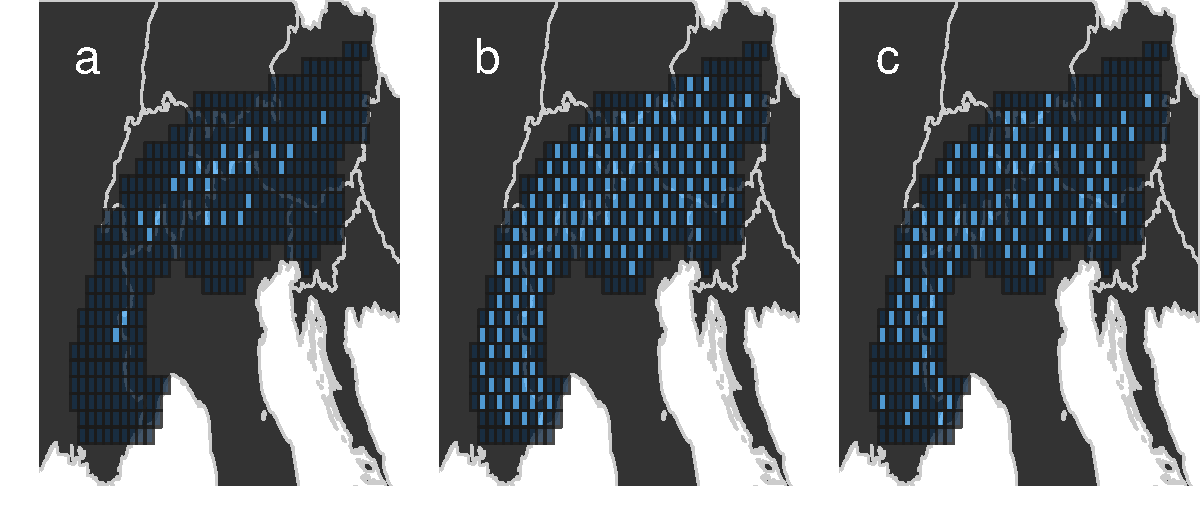
\includegraphics[width=3.42in,height=2.5in]{article_files/figure-latex/unnamed-chunk-3-1.pdf} 

}

\caption{The proportion of adaptive (a; 10 species) and neutral (b; 27 species) genetic variation represented in a suite of randomly generated prioritizations for different species as a function of the surrogate variation they also secured (lines). Panels (c) and (d) show the distribution of $R^2$ values for the 37 models shown in (a) and (b).}\label{fig:unnamed-chunk-3}
\end{figure}

To determine whether environmental and geographic targets could improve
the effectiveness of prioritizations in representing genetic variation,
we generated prioritizations using (i) ``amount targets'' reflecting the
traditional approach of representing a certain proportion of each
species' geographic distribution, (ii) ``amount and surrogate targets''
where we targeted representation of the environmental and geographic
surrogates as well as a certain proportion of each species' geographic
distribution, and (iii) ``amount and genetic targets'' where we targeted
representation of the directly measured genetic variation as well as a
certain proportion of each species' geographic distribution. To
determine if these patterns were robust, for each of the three
combinations of the targets, we generated prioritizations under four
scenarios: (i) single-species with equal costs, (ii) single species with
acquisition costs, (iii) multi-species with equal costs, and (iv)
multi-species with acquisition costs (Figure S30).

\begin{figure}

{\centering 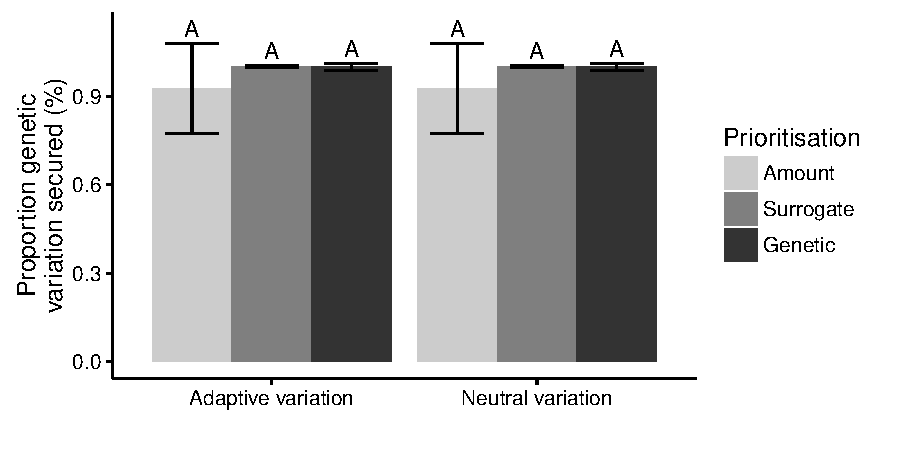
\includegraphics[width=3.42in,height=4in]{article_files/figure-latex/unnamed-chunk-4-1.pdf} 

}

\caption{The proportion of adaptive and neutral genetic variation secured for each species in solutions based on different targets and scenarios. Box plots show the median, and the 25th and 75th percentiles. Whiskers show the data at 1.5 times the inter-quantile range. Points show data outside the whiskers. Red lines show the target proportion of genetic variation.}\label{fig:unnamed-chunk-4}
\end{figure}

The proportion of genetic variation secured in a prioritization depended
on the targets used to generate the prioritization
(\({\chi^2}_{2} = 67.81\); \(P < 0.001)\). Most notably, prioritizations
based on the surrogate variables represented significantly more genetic
variation than amount-based prioritizations (93.24 \% \(\pm\) 13.79 SD
overall genetic variation secured versus 78.33 \% \(\pm\) 23.62 SD;
\(Z_1 = 4.59\); \(P < 0.001\)), and were not distinguishable from
prioritizations based on measured genetic data (94.7 \% \(\pm\) 3.8 SD;
\(Z_1 = 0.56\); \(P > 0.99\)). These results indicate that environmental
and geographic surrogates in this case far outperform traditional
amount-based conservation planning, and perform almost as well as a
conservation plan based directly on measured genetic data.

Overall, the prioritizations tended to secure a greater proportion of
adaptive genetic variation than neutral genetic variation (adaptive:
mean 96.04 \% \(\pm\) 7.61 secured across all prioritizations, neutral:
mean 71.94 \(\pm\) 24.16; \({\chi^2}_{1} = 1408.16\); \emph{P}
\textless{} 0.001). Thus, regardless of the targets used to generate a
prioritization, or the planning context under which the prioritization
was generated, prioritizations tend to secure more adaptive than neutral
genetic genetic variation.

The average proportion of genetic variation secured by prioritizations
varied under different scenarios (\({\chi^2}_{3} = 34.45\); \emph{P}
\textless{} 0.001). Specifically, prioritizations generated under
single-species scenario (mean 78.36 \% genetic variation secured \(\pm\)
23.61) secured less genetic variation than those under the single
species with opportunity costs (mean 88.89 \% genetic variation secured
\(\pm\) 15.52; \(Z_1 = 2.94\); \(P = 0.02\)) or the multi-species with
cost scenarios (mean 91.89 \% genetic variation secured \(\pm\) 12.31;
\(Z_1 = 3.68\); \(P = 0.001\)). These results suggest the amount of
genetic variation secured in a prioritization may be affected by the
data used to represent acquisition cost.

\section*{Discussion}\label{discussion}
% \addcontentsline{toc}{section}{Discussion}

We have shown that broad-scale environmental and geographic variables
can be effective as surrogates for adaptive and neutral genetic
variation in conservation planning. Our study is the first to show this
using field measurements of genetic variation for a broad range of
species. The spatial patterns of environmental and geographic surrogates
were strongly correlated with the patterns of adaptive and neutral
genetic variation for most species. Moreover, for most species,
prioritizations generated using environmental and geographic targets
secured a greater proportion of adaptive and neutral genetic variation
than traditional conservation planning. These environmental and
geographic surrogates were based on freely available data, and could be
applied to any study region across the world.

Our results demonstrate that environmental and geographic variables are
effective surrogates for most species considered here (Figure 2).
Despite this, geographic distance was a suprisingly poor surrogate for
neutral genetic variation for a few species (eg. \emph{Gypsophila
repens}: \(R^2\) = 0.26; \emph{Luzula alpinopilosa}: \(R^2\) = 0.28;
\emph{Gentiana nivalis} \(R^2\) = 0.29). One explanation for this result
is that geographic distance will be a poor surrogate for neutral genetic
variation where spatial genetic structure is complicated by additional
factors (21, 23). For example, some species can maintain relatively high
connectivity between distant populations (eg. wind dispersing plants;
22), and in some places can be disrupted by landscape features (eg.
anthropogenically modified land 21). Overall, such species were the
exception in our analysis, and both surrogates performed moderately well
for most species.

Our results show that environmental and geographic surrogates can be
used to capture genetic variation in prioritizations, the next question
is: what percentage of surrogate variation should planners target to
preserve genetic variation? To secure at least 90 \% of the species'
neutral genetic variation, prioritizations needed to sample 95.07 \%
\(\pm\) 6.1 SD of the variation in geographic position among the
planning units occupied by each species. Additionally, to secure at
least 90 \% of each species' adaptive genetic variation, prioritizations
needed to sample 56.43 \% \(\pm\) 7.54 SD of the environmental variation
in planning units occupied each the species. For all species, however,
it was possible to generate solutions that secured a large proportion of
the surrogate variation (\textgreater{} 90 \%) and only a small
proportion of genetic variation (\textless{} 20 \%; Figures S56--S57).
Planners may avoid such outcomes by using both amount- and
surrogate-based targets. Depending on the study area and the species of
conservation interest, higher targets may be needed to increase the
likelihood that prioritizations will secure a large proportion of the
intra-specific genetic variation for all of the species in the planning
exercise.

Our results suggest that conservation planners can secure a reasonably
representative sample of the intra-specific adaptive genetic variation
using only amount-based targets (Figure 2). For most species, the
spatial patterns of adaptive genetic variation clustered into a few
distinct groups (eg. \emph{Carex sempervirens} and \emph{Cerastium
uniflorum}; Figures S33 and S34 respectively). As a consequence, a
prioritization would only need to select a single planning unit in each
cluster to secure a representative sample. This mechanism explains why
adaptive variation accumulated much more quickly than neutral genetic
variation in the randomly generated prioritizations. Additionally, this
mechanism also explains why the single-species prioritizations generated
using only amount targets were often able to achieve high
representation---they were essentially a random selection and so
frequently contained planning units in different parts of the species'
ranges (Figure 4a). Overall---and contrary to our original
hypothesis---it seems that conventional reserve selection methods might
often conserve species' adaptive genetic variation.

There are several limitations associated with our analysis. Firstly, the
size of the planning units we used (approx. 23 \(\times\) 25 km) is much
larger than typically used in regional conservation planning (1--10
km\(^2\)). We used this resolution because the genetic data were
collected at this scale. Whilst we could have interpolated the genetic
data to a finer resolution and used smaller planning units, this would
have biased our analysis by artificially introducing additional spatial
auto-correlation. Secondly, we used geographic distances as surrogates
for neutral genetic variation, yet distances that incorporate data on
topography may better describe connectivity in the study area. However,
such distances often require species-specific scaling (eg. 21), and so
cannot easily be utilized in multi-species planning exercises. Thirdly,
we used amplified fragment length polymorphism data (AFLP; 24) to
describe genetic variation. Whilst next-generation sequencing provides
higher resolution genetic information than AFLP data (11), we know of no
suitable multi-species genomic data set, and our methodology would still
have utilized only the main gradients of the genetic variation to
generate prioritizations in a feasible period of time. Furthermore, even
with modern population genomic approaches, a survey can at best hope to
identify markers that are linked to functionally adaptive variants.

Broad-scale environmental and geographic variables are generally
effective surrogates for representing adaptive and neutral genetic
variation for most species in our study system. Moreover, data to
calculate the surrogate variables are freely available for any location
in the world. Careful use of such surrogates in conservation planning
could vastly improve the chances of long-term biodiversity persistence
for relatively little additional cost.

\section*{Materials and Methods}\label{materials-and-methods}
% \addcontentsline{toc}{section}{Materials and Methods}

\subsection*{Study system}\label{study-system}
% \addcontentsline{toc}{subsection}{Study system}

We used data for 27 alpine plant species in the European Alps collected
by the IntraBioDiv project (22; Figure 3a). All data, code, and results
are stored in an online repository to permit replication and validation
of this study (\url{www.github.com/jeffreyhanson/genetic-surrogates}).
This data set has been used to explore patterns of adaptive (eg. 25) and
neutral genetic variation (eg. 26), and the potential for species
richness as a surrogate for genetic diversity (27). Data were collected
using a \(20^{\prime}\) longitude by \(21^{\prime}\) latitude grid
(approx. 22.3 \(\times\) 25 km; Figure S31). Project surveyors visited
every second grid cell, and for each species, they collected samples
from three individuals if any individuals were found. They genotyped
samples using AFLPs, and constructed matrices denoting the presence of
polymorphisms at loci for each species (mean 130.7 \(\pm\) 54.9 SD
markers genotyped per species; for more information see 26, Table 1).
Thus the data set contains information describing the genomic properties
of individuals for each species over a geographic grid. We used these
data because they comprised comparable genetic information for a range
of species with different evolutionary and life histories collected
using a standardized sampling scheme.

\begin{figure}

{\centering 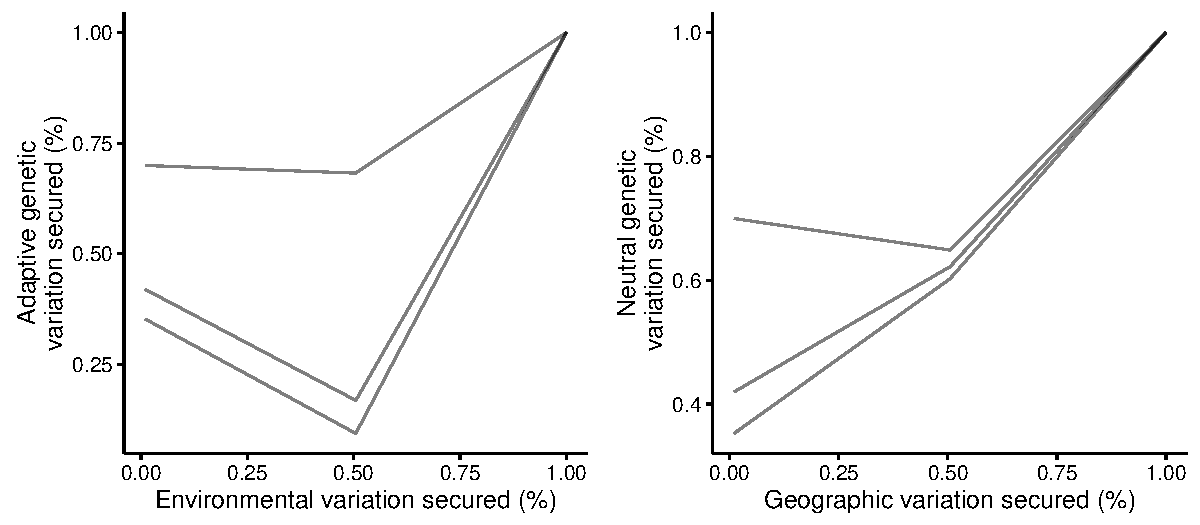
\includegraphics[width=3.42in]{article_files/figure-latex/unnamed-chunk-5-1.pdf} 

}

\caption{Map of the study area showing (a) the pattern of species richness, and (b) the distribution of acquisition cost, both plotted on a quantile-based color ramp. Squares denote planning units.}\label{fig:unnamed-chunk-5}
\end{figure}

\subsection*{Landscape data}\label{landscape-data}
% \addcontentsline{toc}{subsection}{Landscape data}

We adopted the sampling grid used to collect data as planning units to
develop prioritizations. To reduce computational burden, we omitted
cells that did not contain samples (149 grid cells used in analysis). To
examine the effect of variation in cost, we calculated the total human
population density inside each planning unit (1 km\(^2\) resolution from
the Global Rural-Urban Mapping Project; 28) and used this to represent
acquisition cost (Figure 3b). All spatial and statistical analyses were
conducted in \texttt{R} (version 3.3.2; 29).

We created environmental and geographic surrogate variables for each
species (Figure S32). To describe the geographic location of each
planning unit (Figure S33), we projected the grid into an equi-distant
coordinate system (Europe Equidistant Conic; \(\texttt{ESRI:102031}\)),
calculated the centroid of each grid cell, and extracted their
two-dimensional coordinates. To describe the environmental
characteristics of each planning unit (Figure S34), we obtained 19
climatic layers (\(30^{\prime\prime}\) resolution; 30), projected them
and the planning units into an equal-area coordinate system (Europe
Lambert Conformal Conic; \(\texttt{ESRI:102014}\)), and computed
planning unit averages for each climatic variable. To reduce
dimensionality, for each species, we subjected the climatic values
associated with the planning units they were found in to a principal
components analysis (PCA; Table S1). We used the first three principal
components to characterize climatic variation found across the species'
geographic distributions inside the study area (capturing 90.26 \%
\(\pm\) 0.99 SD of the total climatic variation; Figure S2). Thus we
constructed a two-dimensional geographic space as a potential surrogate
for neutral genetic variation, and a three-dimensional environmental
space as a potential surrogate for adaptive genetic variation for each
species. In these spaces, each planning unit was associated with a
single point. Planning units with more comparable environmental
conditions, or higher spatial proximity in the real world, were
associated with points that were closer together in these environmental
or geographic spaces.

\subsection*{Adaptive and neutral genetic
data}\label{adaptive-and-neutral-genetic-data}
% \addcontentsline{toc}{subsection}{Adaptive and neutral genetic data}

To investigate the effectiveness of our putative surrogates, we first
needed to identify which of the sampled loci were adaptive (Figure S35).
Following best practice, we used two outlier detection methods to
achieve this (an individual- and a population-level method; 31). The
basic premise underpinning such methods is that neutral loci are
expected to exhibit a certain level of variation, and loci that deviate
from this expectation are likely to be under selection (11). The
advantage of these methods---in contrast with environmental association
analyses---is that they do not use environmental data, which would have
introduced an element of circularity into our analysis and invalidated
it. Loci identified by both outlier detection methods were treated as
adaptive and the remainder were treated as neutral. To minimize
false-positives, we omitted loci from both methods where the global
frequency of the minor allele was less than 10 \% and treated them as
neutral.

The first outlier detection method involved fitting
multinominal-Dirichlet models implemented in \texttt{BayeScan} (version
2.1; 12). We adopted a similar methodology to Bothwell \emph{et al.}
(25) and applied it to each of the species separately. Following their
methodology, we initially grouped conspecifics into genetic lineages to
further minimize false-positives (Figures S36--S62), by fitting
admixture and correlated alleles models implemented in
\texttt{Structure} (version 2.3.4; 32; 20 replicates per species; 5,000
admixture burnin iterations; 300,000 burnin iterations; 400,000 total
iterations) using the number of lineages previously determined by
Alvarez \emph{et al.} (26) and combining replicate runs using
\texttt{ClumPP} (version 1.1.2; 33; greedy algorithm based on the
\(G^{\prime}\) statistic; 1,000 iterations). We then ran
\(\texttt{Bayescan}\) for each species using these lineages (1:1 prior
odds; 4 replicates per species; 20 pilot runs; 100,000 burn-in
iterations; 110,000 total iterations thinned by 10 iterations) using a
suitable false discovery rate (\(q \leq 0.1\); 34). We omitted
individuals if their population membership was uncertain (maximum
membership probability \(< 0.75\)).

The second outlier detection method involved fitting PCAs to identify
outlier loci (implemented in the \texttt{pcadapt R} package; 13). To
enable comparisons between the two outlier detection methods, we used
the same individuals in this analysis as in the \texttt{BayeScan}
analysis. For each of the 27 species, we first imputed missing data by
replacing missing values with the average frequency among conspecifics,
then ran a PCA over the loci matrix, and extracted the minimum number of
components needed to secure the over-arching population level variation
among the loci (10 \% of the variation in loci). We then computed
\emph{q}-values using Mahalanobis distances, and used the same false
discovery rate used in the \texttt{BayeScan} analysis to identify loci
under selection (using the \texttt{qvalue R} package; 35).

After classifying loci as adaptive or neutral, we mapped the main
gradients of the adaptive (if detected) and neutral genetic variation
for each species. We discarded the population groupings, and partitioned
species' adaptive and neutral loci into separate matrices. We applied
NMDS (implemented in the \texttt{vegan R} package; 36) using Gower
distances (via the \texttt{cluster R} package; 37) to derive continuous
variables that described the main gradients of adaptive and neutral
genetic variation separately for each species (Table S2). To ensure that
the ordinations described a sufficient amount of the genetic variation,
we ran successive scaling analyses with increasing dimensionality until
a sufficient stress value was obtained (maximum stress value \(\leq\)
0.25; 100 random starts for each analysis). Since each grid cell had
multiple samples per species, we averaged the ordinated values for
conspecifics in the same grid cell.

Thus we constructed an adaptive (if detected) and neutral genetic space
for each species. For a given species, each planning unit in which it
occurred was associated with a multi-dimensional point in the species'
adaptive genetic space (if adaptive genetic variation was detected) and
another multi-dimensional point in the species' neutral genetic space.
Planning units that were closer together in these genetic spaces were
occupied by individuals with more comparable AFLP polymorphisms. By
spreading out conservation effort across these genetic spaces, and in
turn selecting planning units occupied by individuals with increasingly
different polymorphisms, prioritizations can secure more genetic
variation.

\subsection*{Prioritization method}\label{prioritization-method}
% \addcontentsline{toc}{subsection}{Prioritization method}

We used the \texttt{raptr R} package to generate solutions (38). This
toolkit can identify the cheapest set of planning units required to
preserve both a target proportion of the species' geographic range
(using amount-based targets) and a broad sample of variation found
across the species' range. We used the environmental and geographic
surrogate spaces, and the adaptive (if detected) and neutral genetic
spaces to generate and evaluate solutions. Solutions associated with
negative values---because they secured very little genetic
variation---were replaced with zeros to facilitate statistical analysis.
We solved all reserve selection problems to within 10 \% of optimality.

\subsection*{Computational and statistical
analyses}\label{statistical-analyses}
% \addcontentsline{toc}{subsection}{Computational and statistical
% analyses}

Our first aim was to determine if the environmental and geographic
variables correlate with the spatial patterns of adaptive and neutral
genetic variation. To achieve this, for each species, we created
dissimilarity matrices using Euclidean distances and the data in the
surrogate and genetic spaces. These matrices showed differences between
the planning units occupied by the species in terms of the units' (i)
geographic position, (ii) environmental characteristics, and the (iii)
adaptive (if detected) and (iv) neutral genetic characteristics of the
individuals inside them.

We fitted maximum likelihood population-effects (MLPE) models using
maximum likelihood to investigate correlations between the dissimilarity
models (using the \texttt{lme4 R} package; 39). These models use random
effects to accommodate the structure of dissimilarity matrices. For each
species, we fitted a MLPE model to the species' dissimilarity matrices
based on geographic position and neutral genetic variation. If adaptive
loci were detected, we also fitted a MLPE model to the species'
dissimilarity matrices describing environmental and adaptive genetic
variation. All data variables were \emph{z}-transformed to improve
convergence. To test if the surrogates explained the genetic variation,
we compared each model to its null model using a \(\chi^2\) test, and
applied Bonferroni corrections.

Our second aim was to determine if the environmental and geographic
variables were effective surrogates for adaptive and neutral genetic
variation. For each species, we generated 20,000 prioritizations by
randomly selecting different combinations of planning units that the
species occupied. For half of these random prioritizations, we
calculated the proportion of geographic variation and neutral genetic
variation they secured, and for the other half, we calculated the
proportion of environmental variation and adaptive genetic variation
they secured. The proportion of surrogate and genetic variation captured
in a prioritization was calculated using the \texttt{raptr R} package.

We fitted two full generalized linear models (GLM) with logit links. The
first model was fit to the proportion of adaptive genetic variation
secured in a prioritization using the proportion of environmental
variation also secured in the prioritization. The second model was fit
to the proportion of neutral genetic variation secured in a
prioritization using the proportion of geographic variation also secured
in the prioritization. Additionally, both models contained a variable
indicating the species for which the prioritizations were generated, and
an interaction term. They were subjected to backwards stepwise term
deletion routines to assess term significance. To assess the performance
of the surrogates, we refit these models separately for each species and
computed the Cragg and Uhler's pseudo-\(R^2\) value (using the
\texttt{pscl R} package; 40).

Our third aim was to determine if surrogate-based targets improved
representation of genetic variation in prioritizations. As previously
mentioned, we generated prioritizations using different combinations of
targets and conservation planning scenarios. We used 20 \% amount-based
targets for each species in all prioritizations to secure an adequate
proportion of the species' distributions. Based on the results from our
previous analysis, we used 97.5 \% surrogate-based targets and 90 \%
genetic-based targets. We generated a single solution for each
target/scenario combination, except for the ``single-species (equal
costs) with amount-based targets'' combination for which we generated
1,000 replicates because it had many optimal solutions. We computed the
proportion of adaptive (if present) and neutral genetic variation
secured for each species in the prioritizations.

We fitted generalized linear mixed-effects models (GLMMs) with logit
links to evaluate the prioritizations (using the \texttt{lme4 R}
package). We fitted a full model to the proportion of genetic variation
secured in a given prioritization. This model contained categorical
variables indicating the targets (amount only, amount and surrogate
targets, or amount and genetic targets), the planning scenario
(single-species, multi-species, or multi-species with cost), the type of
genetic variation measured (adaptive or neutral), and all interactions
between them. Data for same species were accommodated using a random
intercept term. The full model was subjected to a backwards stepwise
term deletion routine to assess significance. A \emph{post-hoc} analysis
was conducted on the minimal adequate model using Tukey contrasts with a
Bonferroni correction (using the \texttt{multcomp R} package; 41).

\showmatmethods
\showacknow
\pnasbreak

\begin{thebibliography}{100}
\bibitem{r440}
Sanderson EW, Segan DB, Watson JEM (2015) Global status of and
prospects for protection of terrestrial geophysical diversity.
\emph{Conserv Biol} 29(3):649--656.

\bibitem{r255}
Margules CR, Pressey RL (2000) Systematic conservation planning.
\emph{Nature} 405(6783):243--253.

\bibitem{r9}
Cowling RM, Pressey RL (2001) Rapid plant diversification: Planning
for an evolutionary future. \emph{Proc Natl Acad Sci USA}
98(10):5452--5457.

\bibitem{r165}
Hendry AP, et al. (2011) Evolutionary principles and their practical
application. \emph{Evol Appl} 4(2):159--183.

\bibitem{r504}
Fournier-Level A, et al. (2016) Predicting the evolutionary dynamics
of seasonal adaptation to novel climates in arabidopsis thaliana.
\emph{Proc Natl Acad Sci USA} 113(20):E2812--E2821.

\bibitem{r67}
Moritz C (1999) Conservation units and translocations: Strategies for
conserving evolutionary processes. \emph{Hereditas} 130(3):217--228.

\bibitem{r3}
Crandall KA, Bininda-Emonds ORP, Mace GM, Wayne RK (2000) Considering
evolutionary processes in conservation biology. \emph{Trends Ecol Evol}
15(7):290--295.

\bibitem{r499}
Rosauer D, Laffan SW, Crisp MD, Donnellan SC, Cook LG (2009)
Phylogenetic endemism: A new approach for identifying geographical
concentrations of evolutionary history. \emph{Mol Ecol}
18(19):4061--4072.

\bibitem{r61}
Hendry AP, et al. (2010) Evolutionary biology in biodiversity
science, conservation, and policy: A call to action. \emph{Evolution}
64(5):1517--1528.

\bibitem{r503}
Carvalho SB, et al. (2017) Spatial conservation prioritization of
biodiversity spanning the evolutionary continuum. \emph{Nat Ecol Evol}
1(1):0151.

\bibitem{r480}
Schoville SD, et al. (2012) Adaptive genetic variation on the
landscape: Methods and cases. \emph{Annu Rev Ecol Evol S} 43:23--43.

\bibitem{r456}
Foll M, Gaggiotti O (2008) A genome-scan method to identify selected
loci appropriate for both dominant and codominant markers: A bayesian
perspective. \emph{Genetics} 180(2):977--993.

\bibitem{r487}
Duforet-Frebourg N, Bazin E, Blum MG (2014) Genome scans for
detecting footprints of local adaptation using a bayesian factor model.
\emph{Mol Biol Evol} 31(9):2483--2495.

\bibitem{r500}
Steiner JNAH Cynthia C AND Weber (2007) Adaptive variation in beach
mice produced by two interacting pigmentation genes. \emph{PLoS Biol}
5(9):1--10.

\bibitem{r43}
Sgro CM, Lowe AJ, Hoffmann AA (2011) Building evolutionary
resilience for conserving biodiversity under climate change. \emph{Evol
Appl} 4(2):326--337.

\bibitem{r2}
Carvalho SB, Brito JC, Crespo EJ, Possingham HP (2011) Incorporating
evolutionary processes into conservation planning using species
distribution data: A case study with the western mediterranean
herpetofauna. \emph{Divers Distrib} 17(3):408--421.

\bibitem{r200}
Ponce-Reyes R, Clegg SM, Carvalho SB, McDonald-Madden E, Possingham
HP (2014) Geographical surrogates of genetic variation for selecting
island populations for conservation. \emph{Divers Distrib}
20(6):640--651.

\bibitem{r202}
Rouget M, Cowling RM, Pressey RL, Richardson DM (2003) Identifying
spatial components of ecological and evolutionary processes for regional
conservation planning in the cape floristic region, south africa.
\emph{Divers Distrib} 9(3):191--210.

\bibitem{r501}
Avise JC (2009) Phylogeography: Retrospect and prospect. \emph{J
Biogeogr} 36(1):3--15.

\bibitem{r259}
Wright S (1943) Isolation by distance. \emph{Genetics}
28(2):114--138.

\bibitem{r497}
Dudaniec RY, et al. (2016) Dealing with uncertainty in landscape
genetic resistance models: A case of three co-occurring marsupials.
\emph{Mol Ecol} 25(2):470--486.

\bibitem{r451}
Meirmans P, Goudet J, IntraBioDiv Consortium, Gaggiotti O (2011)
Ecology and life history affect different aspects of the population
structure of 27 high-alpine plants. \emph{Mol Ecol} 20(15):3144--3155.

\bibitem{r505}
Fortuna MA, Albaladejo RG, Fernández L, Aparicio A, Bascompte J
(2009) Networks of spatial genetic variation across species. \emph{Proc
Natl Acad Sci USA} 106(45):19044--19049.

\bibitem{r453}
Vos P, et al. (1995) AFLP: a new technique for DNA fingerprinting.
\emph{Nucleic Acids Res} 23(21):4407--4414.

\bibitem{r455}
Bothwell H, et al. (2013) Identifying genetic signatures of
selection in a non-model species, alpine gentian (\emph{Gentiana nivalis
L.}), using a landscape genetic approach. \emph{Conserv Genet}
14(2):467--481.

\bibitem{r478}
Alvarez N, et al. (2009) History or ecology? Substrate type as a
major driver of patial genetic structure in alpine plants. \emph{Ecol
Lett} 12(7):632--640.

\bibitem{r486}
Taberlet P, et al. (2012) Genetic diversity in widespread species is
not congruent with species richness in alpine plant communities.
\emph{Ecol Lett} 15(12):1439--1448.

\bibitem{r472}
CIESEN, Columbia University, International Food Policy Research
Institute, The World Bank, Centro Internacional de Agricultura Tropical
(2011) Global rural-urban mapping project, Version 1 (GRUMP v1): Urban
extents grid. Available at: \url{http://dx.doi.org/10.7927/H4GH9FVG}.

\bibitem{r192}
R Core Team (2014) R: A language and environment for statistical
computing. Available at: \url{http://www.R-project.org/}.

\bibitem{r33}
Hijmans RJ, Cameron SE, Parra JL, Jones PG, Jarvis A (2005) Very
high resolution interpolated climate surfaces for global land areas.
\emph{Int J Climatol} 25(15):1965--1978.

\bibitem{r495}
Villemereuil P de, Frichot É, Bazin É, François O, Gaggiotti OE
(2014) Genome scan methods against more complex models: When and how
much should we trust them? \emph{Mol Ecol} 23(8):2006--2019.

\bibitem{r462}
Falush D, Stephens M, Pritchard JK (2007) Inference of population
structure using multilocus genotype data: Dominant markers and null
alleles. \emph{Mol Ecol Notes} 7(4):574--578.

\bibitem{r459}
Jakobsson M, Rosenberg NA (2007) CLUMPP: A cluster matching and
permutation program for dealing with label switching and multimodality
in analysis of population structure. \emph{Bioinformatics}
23(14):1801--1806.

\bibitem{r466}
Benjamini Y, Hochberg Y (1995) Controlling the false discovery rate:
A practical and powerful approach to multiple testing. \emph{J Roy Stat
Soc B Met} 57(1):289--300.

\bibitem{r491}
Storey JD, Bass AJ, Dabney A, Robinson D (2015) Qvalue: Q-value
estimation for false discovery rate control. R package version 2.2.2.
Available at: \url{http://github.com/jdstorey/qvalue}.

\bibitem{r458}
Oksanen J, et al. (2015) Vegan: Community ecology package. R package
version 2.3-2. Available at:
\url{http://CRAN.R-project.org/package=vegan}.

\bibitem{r457}
Maechler M, Rousseeuw P, Struyf A, Hubert M, Hornik K (2015)
Cluster: Cluster analysis basics and extensions. R package version
2.0.3. Available at: \url{http://CRAN.R-project.org/package=cluster}.

\bibitem{r465}
Hanson JO, Rhodes JR, Possingham HP, Fuller RA (XXX) raptr:
Representative and adequate prioritization toolkit in R.
\emph{Unpublished} XX(XX):XX--XX.

\bibitem{r469}
Bates D, Mächler M, Bolker B, Walker S (2015) Fitting linear
mixed-effects models using lme4. \emph{J Stat Softw} 67(1):1--48.

\bibitem{r492}
Jackman S (2015) pscl: Classes and Methods for R Developed in the
Political Science Computational Laboratory, Stanford University. R
package version 1.4.9. Available at: \url{http://pscl.stanford.edu}.

\bibitem{r470}
Hothorn T, Bretz F, Westfall P (2008) Simultaneous inference in
general parametric models. \emph{Biometrical J} 50(3):346--363.



% Bibliography
% \bibliography{pnas-sample}

\end{thebibliography}
\end{document}

